\chapter{Implantation De Le Loi De Commande}
      
       
 
 
\addcontentsline{toc}{chapter}{Implantation De Le Loi De Commande}
 \section{Calcul D’un Observateur Minimal Identité}

 \subsection{Le modèle linéarisé est-il observable ?}
 
 Pour voir est ce que le système étudier est observable   on va calculer la matrice de l'observabilté : \\
 Méthode analytique :\\\\
      $obs$=$\begin{bmatrix}
      C & CA & CA^{2}
      \end{bmatrix}^{T}$\\\\
      
      $obs$=$\begin{bmatrix}
      1 & 0 & 0 \\
      -0.2349 & -1.0938 & 0.9174 \\
      0.0451 & 0.2883 & -0.2717 \\
      \end{bmatrix}$
      
De même, on a vérifier avec MATLAB l'observabilité du système. \hyperref[section1.3]{(voir Annexe 3)}\label{annexe3}\\ 

 On remarque que le rang de la matrice obs est égale à la dimension du système d'ou le système est observable.
 %%%%%%%%%%%copmpleter%%%%%%%%
 
 \subsection{Calcul Du Nouveau Observateur identité }
Constitution de l'observateur minimale identité\\\\
$A$=$\begin{bmatrix}
-0.0092 & 0.0092 & 0 \\
0.0092 & -0.0198 & 0.0106\\
0 & 0.0106 & 0.0486\\
\end{bmatrix}$\\\\
Séparation de la matrice A 

$A_{11}=\begin{bmatrix}
-0.0092
\end{bmatrix}
\quad ;
A_{21}=\begin{bmatrix}
0.0092\\
0
\end{bmatrix}$\\\\


$A_{11}=\begin{bmatrix}
0.0092 & 0
\end{bmatrix}
\quad ;
A_{22}=\begin{bmatrix}
-0.0198 & 0.0106 \\
0.0106 & 0.0486
\end{bmatrix}$\\\\
 


\begin{equation}
\left\{\begin{matrix}
\dot{s}(t)=Fs(t)+(FG-GA_{11}+A_{21})y(t)+(B_{2}-GB_{1}u(t))\\
 x^(t)=s(t)+Gy(t)\\
\end{matrix}\right.
\end{equation}   
talque\\ 
$F$=$A_{22}-GA_{12}$\\\\
alors on a \\\\
$\begin{bmatrix}
f_{11} & f_{12}\\
f_{21} & f_{22}\\
\end{bmatrix}
\quad=
\begin{bmatrix}
1 & 1\\
0 & 1\\
\end{bmatrix}
\quad-
\begin{bmatrix}
g1\\
g2\\
\end{bmatrix}
\quad
\begin{bmatrix}
0.0092 & 0
\end{bmatrix}$\\\\

alors on aura \\\\
$F=
\begin{bmatrix}
f_{11} & f_{12}\\
f_{21} & f_{22}\\
\end{bmatrix}
\quad=
\begin{bmatrix}
(1-0.0092g_{1}) & 1\\
(-0.0092g_{2}) && 1\\
\end{bmatrix}$\\\\

puis en calcule  le déterminent de cette matrice puis on va faire l'identification avec le polynôme désiré\\\\

$det(\lambda I-F)= 2-0.0092g_{1}\lambda-0.0092_{g2}$\\

$P_{désiré}=(\lambda+0.11)(\lambda+0.17)\\$
           


par identification on trouve:\\\\

$G=\begin{bmatrix}
0.1393^{3}\\
3.9546^{3}\\
\end{bmatrix}
\quad
F=\begin{bmatrix}
-1.3014 & 0.0106\\
 -36.3807 & -0.0486\\
\end{bmatrix}$\\\\

$Calcule De G_{tild} et H_{tild}$:\\\\

$G_{tild}=FG-GA_{11}+A_{21}
\quad\\\\
G_{tild}=\begin{bmatrix}
-0.0904^{3}\\
 -2.5679^{3}\\
\end{bmatrix}$\\\\
$B_{11}=\begin{bmatrix}
64.9351
\end{bmatrix}
\quad 
B_{21}=\begin{bmatrix}
0\\
0
\end{bmatrix}$


$H_{tild}=B_{21}G-GB_{11}
\quad\\\\
\begin{bmatrix}
-0.0904^{5}\\
 -2.5678^{5}\\
\end{bmatrix}$\\\\

\begin{equation}
\left\{\begin{matrix}
\dot{s}(t)=\begin{bmatrix}
-1.3014 & 0.0106\\
 -36.3807 & -0.0486\\
\end{bmatrix}s(t)+(\begin{bmatrix}
-1.3014 & 0.0106\\
 -36.3807 & -0.0486\\
\end{bmatrix}\begin{bmatrix}
0.1393^{3}\\
3.9546^{3}\\
\end{bmatrix}-\begin{bmatrix}
0.1393^{3}\\
3.9546^{3}\\
\end{bmatrix}A_{11}\\
+A_{21})y(t)+(B_{2}-
\begin{bmatrix}
0.1393^{3}\\
3.9546^{3}\\
\end{bmatrix}B_{1}u(t))\\
 x^(t)=s(t)+\begin{bmatrix}
0.1393^{3}\\
3.9546^{3}\\
\end{bmatrix}y(t)\\
\end{matrix}\right.\\\\
\end{equation}   
On a aussi calculer l'observateur minimal identité avec Matlab \hyperref[section1.3]{(voir Annexe 3)}\label{annexe3}\\
 
 \subsection{Insertion Dans Notre  Schéma Simulink l’observateur sous la forme d’un bloc State-Space avec le bouclage déterminé précésemment.}

\begin{center}
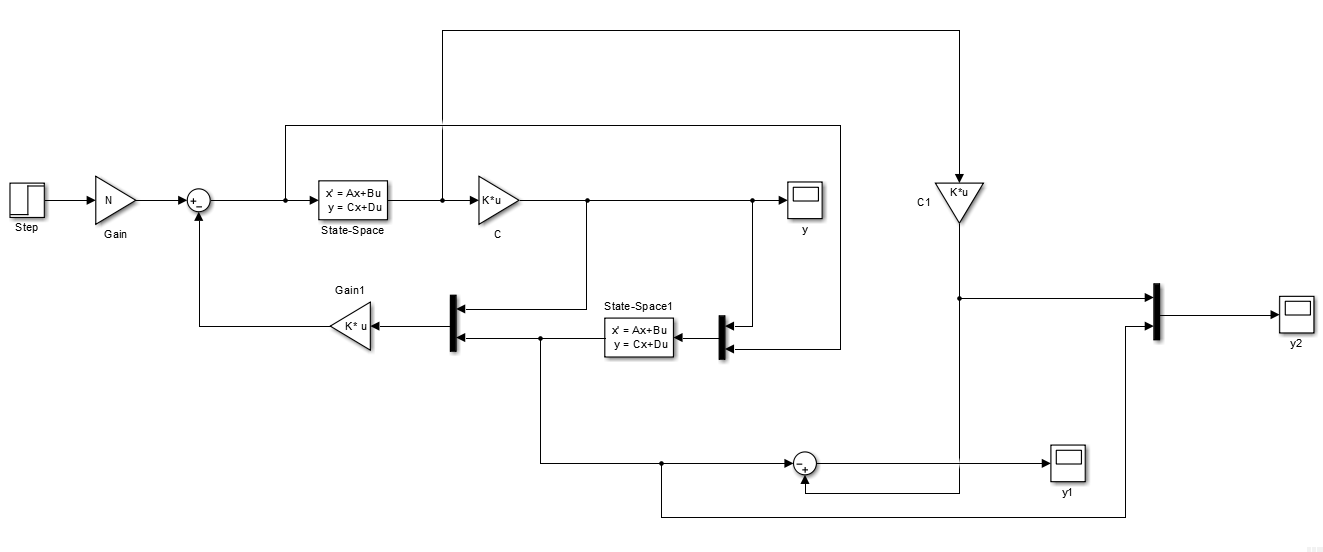
\includegraphics[scale=0.4]{schemabloc2.PNG}
\captionof{figure}{\textit{Schéma simulink avec l'observateur minimal identité.}}
\label{fig1} 
\end{center}   
  
 \subsection{Vérification, que les états estimés convergent vers les états réels du système linéarisé.\\\\} 
 
\begin{center}
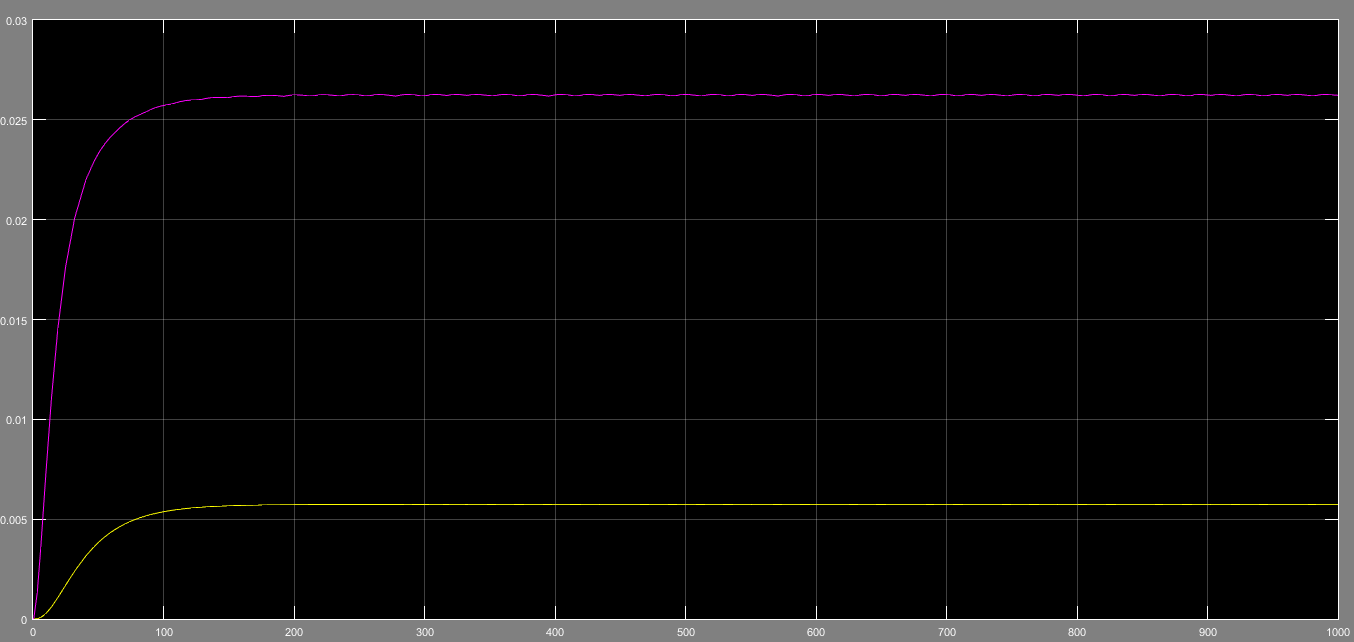
\includegraphics[scale=0.4]{Y1.PNG}
\captionof{figure}{\textit{le tracé des sorties éstimées.}}
\label{fig3} 
\end{center}
 
 Selon la figure au-dessus, on remarque que la courbe de chaque état estimé converge vers son état réel.\\\\  
 
 \subsection{Évaluation De  L’influence des Conditions Initiales.\\\\}

Après avoir changé sur l'observateur minimale construit, ses conditions initiales [0 0] vers [0.5 0.5], sur Simulink on aura le tracé des deux courbes illustrées sur la figure au-dessous :\\    

\begin{center}
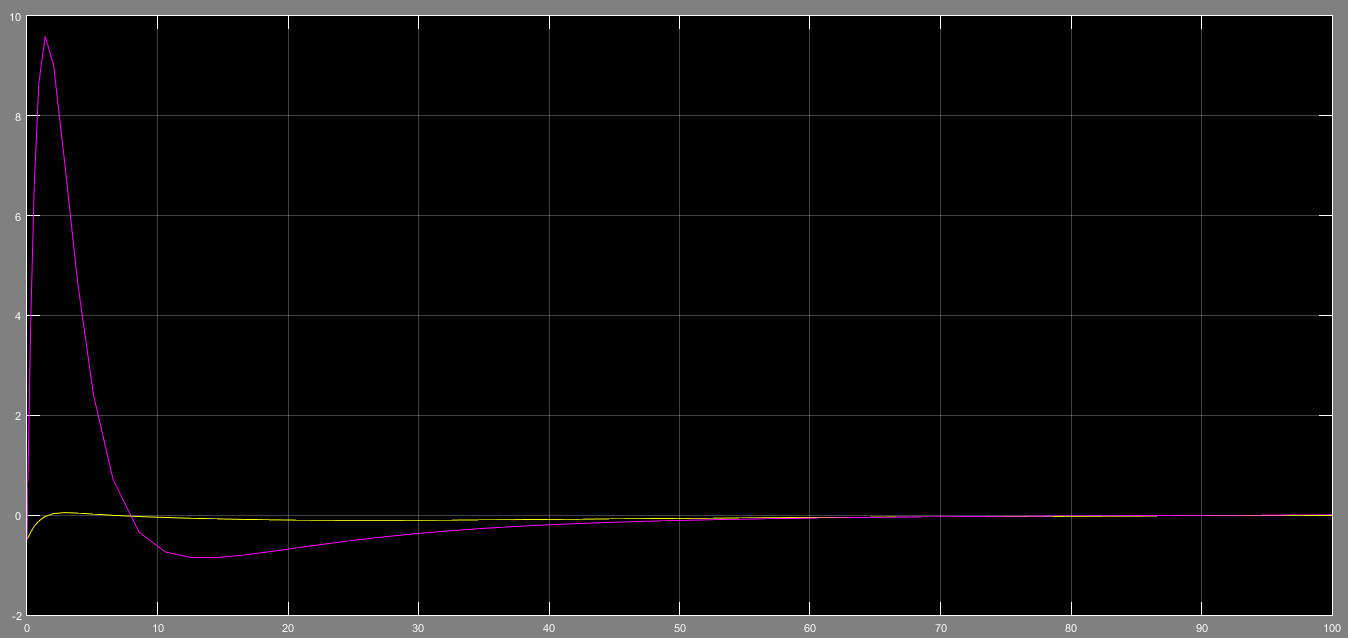
\includegraphics[scale=0.4]{Y1_condi_init.PNG}
\captionof{figure}{\textit{le tracé des sorties éstimées avce les condition initials.}}
\label{fig3} 
\end{center}

  
 \section{Bruit Sur La Sortie Mesurée\\\\}
 
 \begin{center}
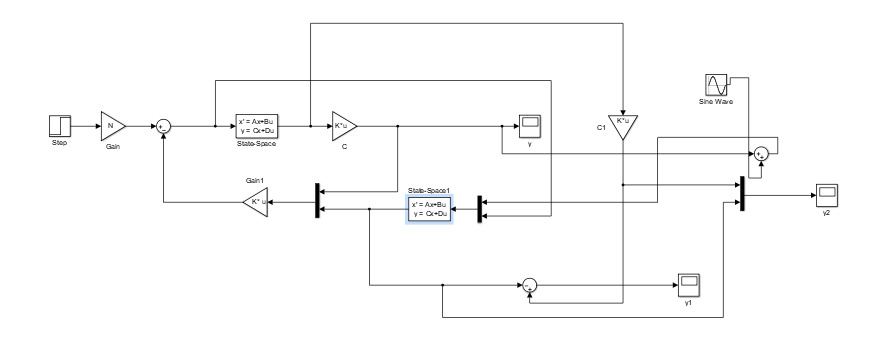
\includegraphics[scale=0.6]{schemabloc_bruit.PNG}
\captionof{figure}{\textit{schéma simulink avec l'ajout de bruit.}}
\label{fig3} 
\end{center}


\begin{center}
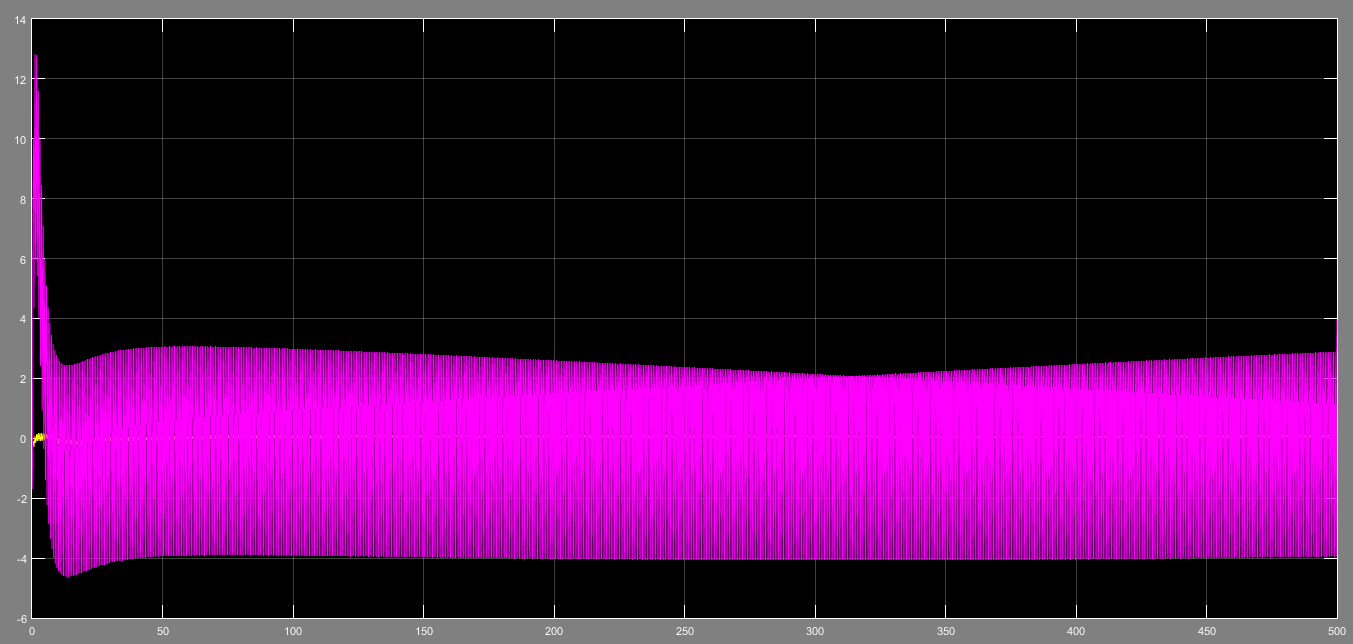
\includegraphics[scale=0.4]{Y1_bruit.PNG}
\captionof{figure}{\textit{le tracé des sorties estimées avec le bruit.}}
\label{fig3} 
\end{center}
 
 

  \subsection{Calcule d'un nouvel observateur de dynamique uniquement 2 fois plus rapide que le système bouclé par le retour d’état.\\\\}

Dans cette partie, on multiplie les deux valeurs propres $P_{2}$ et $P_{3}$ par x2, et on obtient le tracé suivant :   


\begin{center}
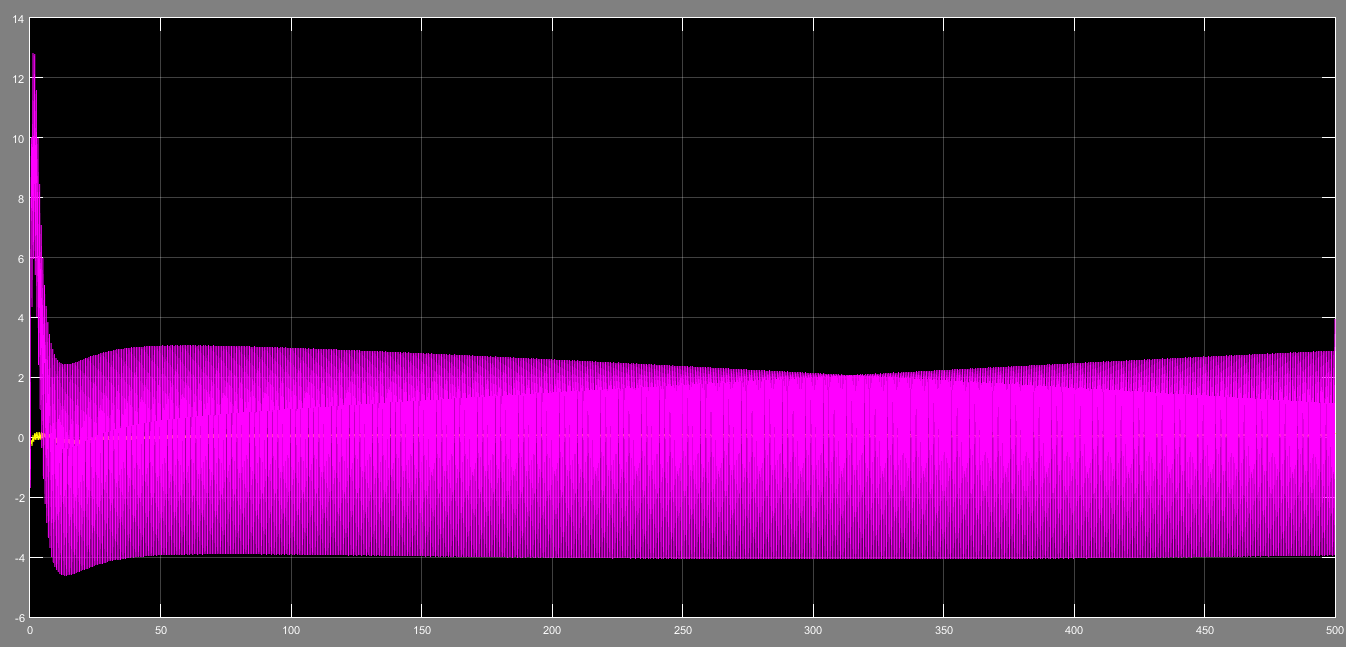
\includegraphics[scale=0.4]{Y1_2P_bruit.PNG}
\captionof{figure}{\textit{le tracé des sorties d'un nouvel observateur de dynamique 2 fois plus rapide que le système bouclé.}}
\label{fig3} 
\end{center}
  
  
  
  
  
  
  
  
  
  